\documentclass{beamer}
\usetheme{Boadilla}

\usepackage{amsmath}
\usepackage{amsfonts}
\usepackage{hyperref}
\usepackage{algorithm}
\usepackage{algpseudocode}


\usepackage{amsmath}
\DeclareMathOperator*{\argmax}{arg\,max}
\DeclareMathOperator*{\argmin}{arg\,min}

\title{The Variational Gaussian Process}
\author{Dmitry Protasov}
\institute{MIPT}

\begin{document}

\begin{frame}
    \titlepage
\end{frame}

\begin{frame}{Introduction}
    \begin{itemize}
        \item Variational inference is a powerful tool for approximate posterior inference.
        \item Traditional methods like mean-field approximation, which assume \textbf{independent distributions for each latent variable}, have limitations in capturing dependencies among them.
        \item \textbf{The Variational Gaussian Process (VGP)} is introduced as a flexible model that adapts to complex posterior distributions.
        \item VGP achieves state-of-the-art results in unsupervised learning, particularly with deep latent Gaussian models and DRAW.
    \end{itemize}
\end{frame}

\begin{frame}{Gaussian processes}
    \begin{itemize}
        \item GP regression estimates the function $f$ given data pairs $\{(s_n, t_n)\}$.
        \item GP prior: $p(f) = \prod \text{GP}(f_i; 0, K_{ss})$ where $K_{ss}$ is the covariance function $k(s, s')$.
        \item ARD kernels: $k(s, s') = \sigma^2_{ARD} \exp\left(-\frac{1}{2} \sum \omega_j (s_j - s'_j)^2\right)$.
        \item Weights $\omega_j$ tune the importance of each dimension and can be driven to zero during inference, leading to automatic dimensionality reduction.
        \item Given data $D$, the conditional distribution of the GP interpolates between input-output pairs:
        \[
        p(f | D) = \prod_{i=1}^d \text{GP}\left(f_i; K_{\xi s} K_{ss}^{-1} t_i, K_{\xi \xi} - K_{\xi s} K_{ss}^{-1} K_{\xi s}^\top\right),
        \]
        where $K_{\xi s}$ is the covariance function $k(\xi, s)$ for input $\xi$ and all data inputs $s_n$.
    \end{itemize}
\end{frame}


\begin{frame}{Variational gaussian process}
    \begin{figure}{}
        \centering
        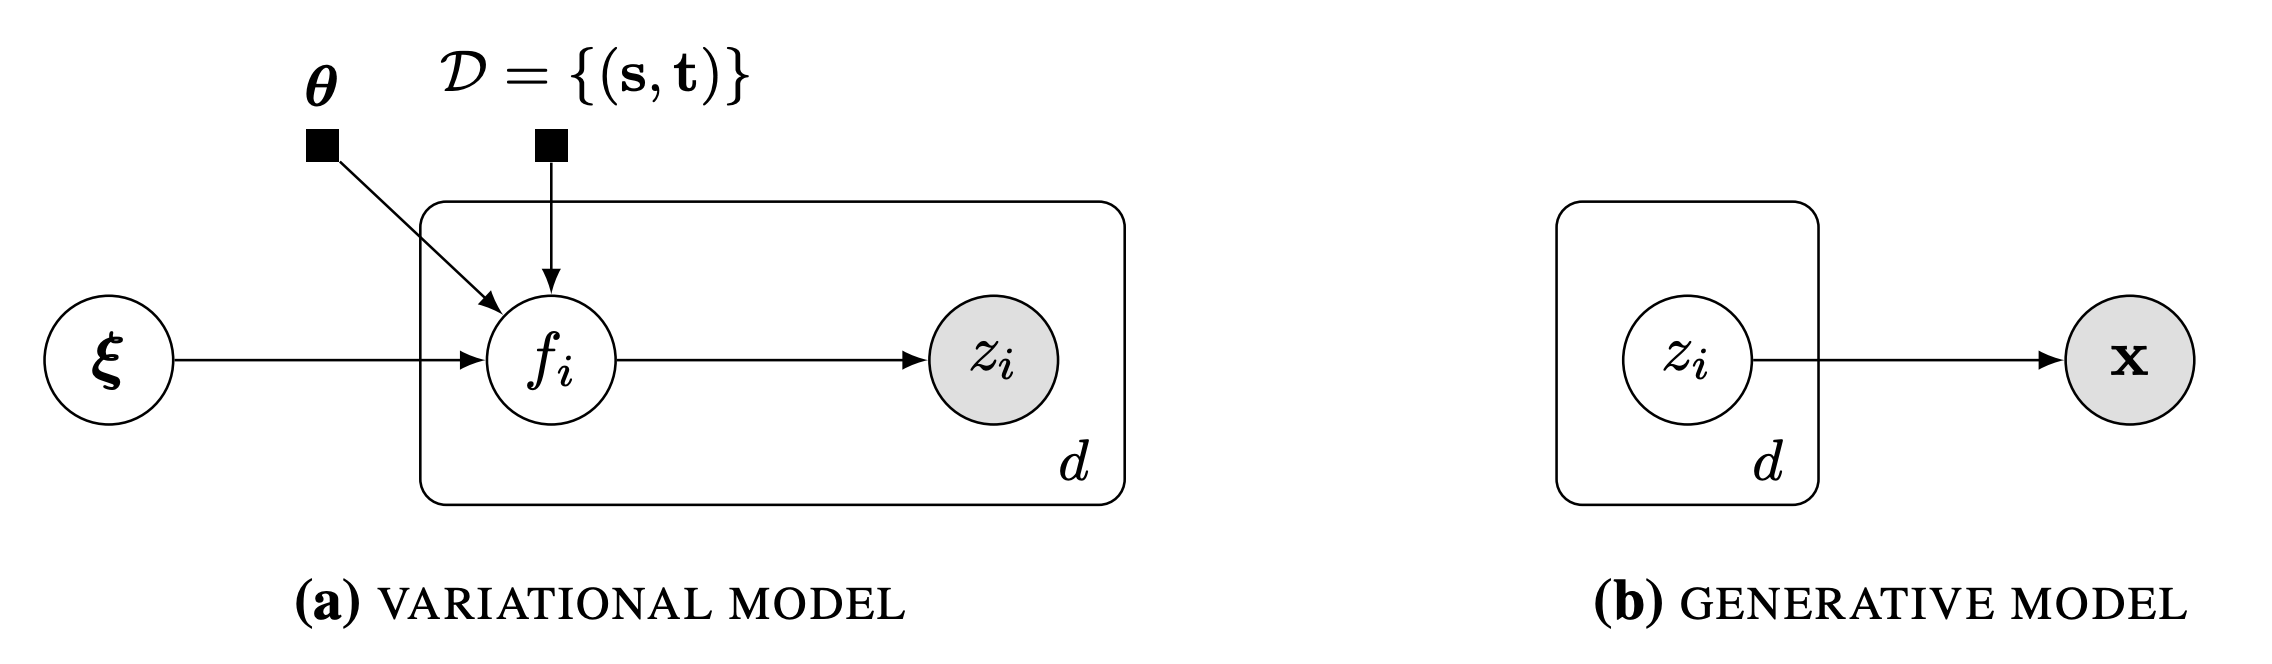
\includegraphics[scale=0.24]{images/figure1a.png}
    \end{figure}

    The VGP specifies the following generative process for posterior latent variables \(z\)

    \begin{itemize}
        \item Draw latent input $\xi \in \mathbb{R}^c$: $\xi \sim \mathcal{N}(0, I)$.
        \item Draw non-linear mapping $f: \mathbb{R}^c \to \mathbb{R}^d$ conditioned on $\mathcal{D}$: $f \sim \prod_{i=1}^d \mathcal{GP}(0, K_{\xi\xi}) \mid \mathcal{D}$.
        \item Draw approximate posterior samples $z \in \text{supp}(p)$: $\mathbf{z} = (z_1, \ldots, z_d) \sim \prod_{i=1}^d q(f_i(\xi))$.
        \item The VGP can capture complex dependencies and correlations between latent variables. VGP is parameterized by kernel hyperparameters $\theta$ and variational data
    \end{itemize}

\end{frame}



\begin{frame}{Universal approximation theorem}
    \begin{block}{Theorem} Let $q(z; \theta, D)$ denote the variational Gaussian process. Consider a posterior distribution $p(z | x)$ with a finite number of latent variables and continuous quantile function (inverse CDF). There exists a sequence of parameters $(\theta_k, D_k)$ such that
        \[
        \lim_{k \to \infty} \text{KL}(q(z; \theta_k, D_k) \| p(z | x)) = 0.
        \]
    \end{block}

    \begin{itemize}
        \item Theorem: any posterior distribution with strictly positive density can be represented by a VGP.
        \item This makes the VGP a flexible model for learning posterior distributions.
    \end{itemize}
\end{frame}


\begin{frame}{Black box inference}
    \begin{figure}{}
        \centering
        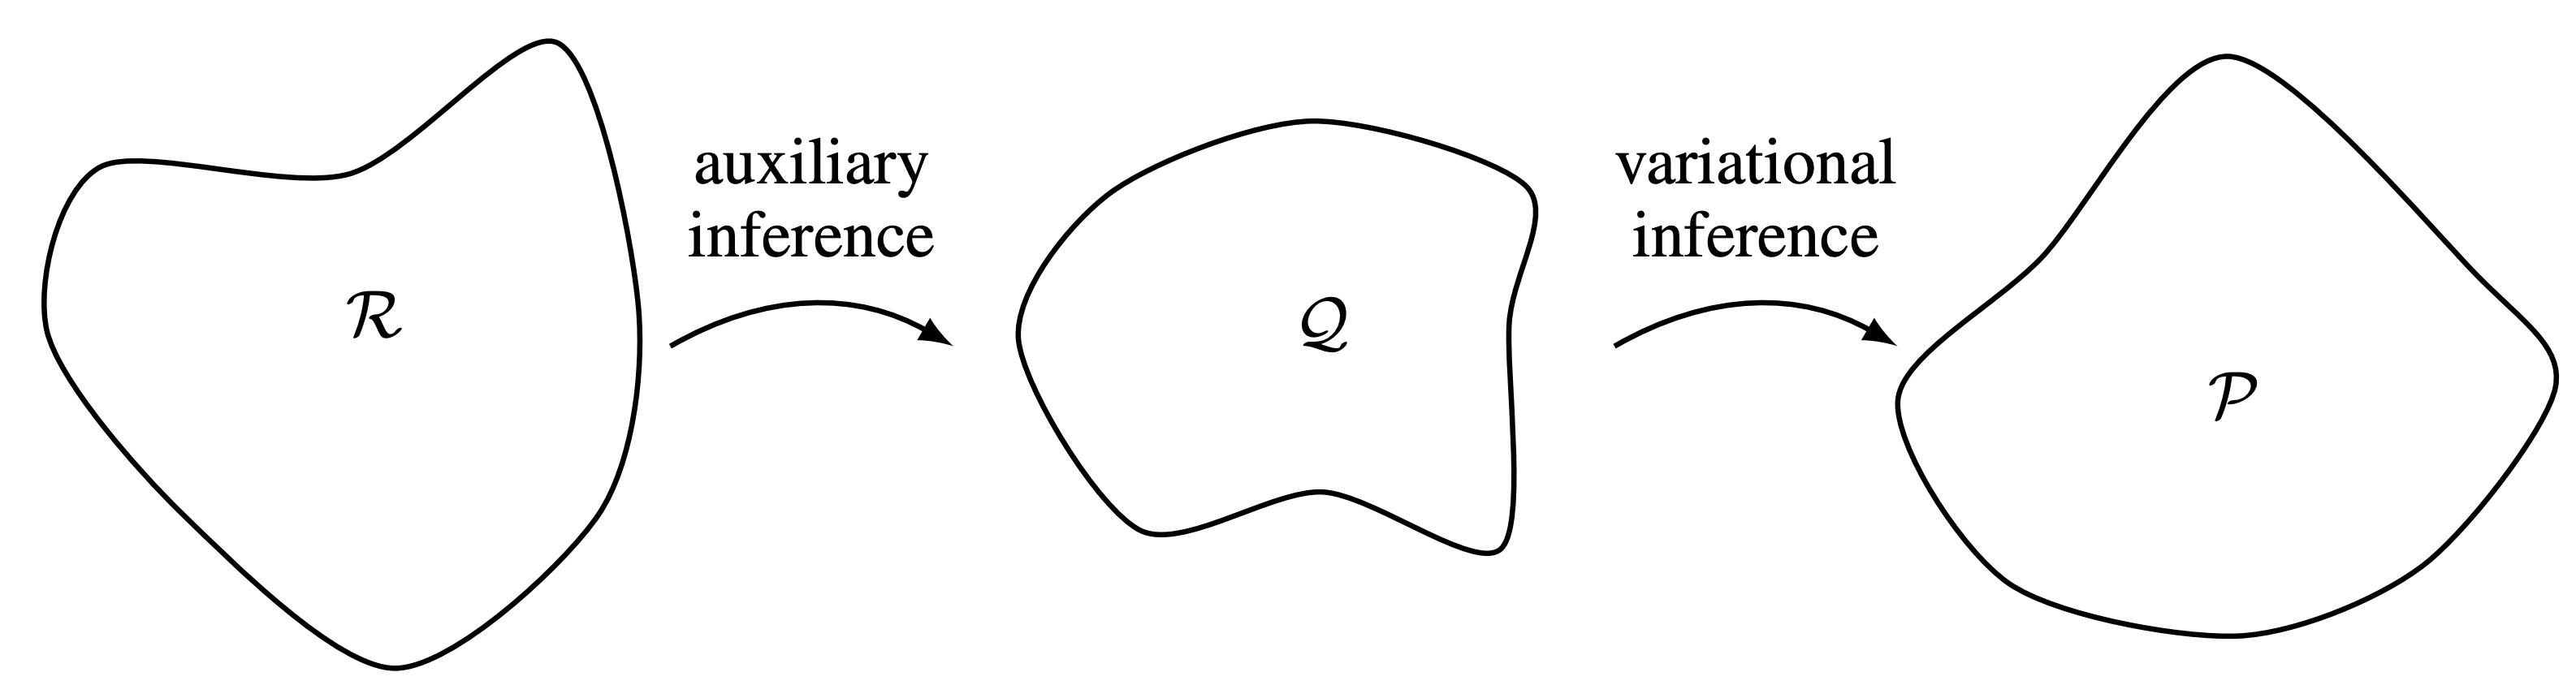
\includegraphics[scale=0.17]{images/figure2.png}
        \caption{Sequence of domain mappings during inference, from variational latent variable space \(\mathcal{R}\) to posterior latent variable space \(\mathcal{Q}\)  to data space \(\mathcal{P}\)}
        \label{fig:enter-label}
    \end{figure}

    Unlike previous approaches, we rewrite this variational objective to connect to auto-encoders:
    \begin{equation}
        \mathcal{L}(\theta, \phi) = & \ \mathbb{E}_{q_{\text{VGP}}} [\log p(\mathbf{x} \mid \mathbf{z})] - \mathbb{E}_{q_{\text{VGP}}} \left[ \text{KL}(q(\mathbf{z} \mid f(\boldsymbol{\xi})) \parallel p(\mathbf{z})) \right] \\
        & - \mathbb{E}_{q_{\text{VGP}}} \left[ \text{KL}(q(f \mid \boldsymbol{\xi}; \theta) \parallel r(f \mid \boldsymbol{\xi}, \mathbf{z}; \phi)) + \log q(\boldsymbol{\xi}) - \log r(\boldsymbol{\xi} \mid \mathbf{z}) \right]
    \end{equation}

    
\end{frame}

\begin{frame}{Black box inference}
\begin{algorithm}[H]
\caption{Black box inference with a variational Gaussian process}
\begin{algorithmic}[1]
    \State \textbf{Input:} Model $p(\mathbf{x}, \mathbf{z})$, Mean-field family $\prod_i q(z_i \mid f_i(\boldsymbol{\xi}))$.
    \State \textbf{Output:} Variational and auxiliary parameters $(\theta, \phi)$.
    \State Initialize $(\theta, \phi)$ randomly.
    \While{not converged}
        \State Draw noise samples $\boldsymbol{\xi} \sim \mathcal{N}(0, \mathbf{I}), \epsilon \sim w$.
        \State Parameterize variational samples $\mathbf{z} = \mathbf{z}(\epsilon; f(\boldsymbol{\xi})), f(\boldsymbol{\xi}) = f(\boldsymbol{\xi}; \theta)$.
        \State Update $(\theta, \phi)$ with stochastic gradients $\nabla_\theta \mathcal{L}, \nabla_\phi \mathcal{L}$.
    \EndWhile
\end{algorithmic}
\end{algorithm}

\begin{itemize}
    \item Algorithm has $O(d + m^3 + LH^2)$ complexity, where $d$ is the number of latent variables, $m$ is the size of variational data, and $L$ is the number of layers in neural networks.
    \item Unlike most GP literature, we require no low rank constraints, such as the use of inducing variables for scalable computation.
\end{itemize}

\end{frame}

\begin{frame}{Related Work and Advantages of VGP}
    \begin{itemize}
        \item VGP vs. Parametric Methods:
        \begin{itemize}
            \item VGP uses a Bayesian nonparametric prior over all continuous mappings.
            \item No need for costly Jacobian determinants ($O(d^3)$ complexity).
            \item Fully Bayesian and flexible over the space of mappings.
        \end{itemize}
        \item Efficiency and Flexibility:
        \begin{itemize}
            \item VGP provides black box inference with lower variance gradients.
            \item Applies location-scale transforms for reparameterization.
            \item Efficient auxiliary inference for variational latent variables.
        \end{itemize}
        \item Classic Techniques and Adaptability:
        \begin{itemize}
            \item Builds on classic Bayesian inference techniques.
            \item VGP adaptively learns transformations, avoiding discretization.
        \end{itemize}
    \end{itemize}
\end{frame}

\begin{frame}{Experiments}
    \begin{itemize}
        \item \textbf{Binarized MNIST}: 
            \begin{itemize}
                \item Deep latent Gaussian model (DLGM) and DRAW used for evaluation.
                \item VGP achieves highest known results on log-likelihood using DRAW (-79.88).
                \item VGP achieves highest known results among non-structure exploiting models using DLGM (-81.32).
            \end{itemize}
        \item \textbf{Sketch Data Set}: 
            \begin{itemize}
                \item DRAW with VGP outperforms original DRAW on Sketch dataset.
                \item Higher visual fidelity and better lower bound on log-likelihood.
            \end{itemize}
    \end{itemize}
    
\end{frame}

\begin{frame}{Experiments}
    \begin{figure}{}
        \centering
        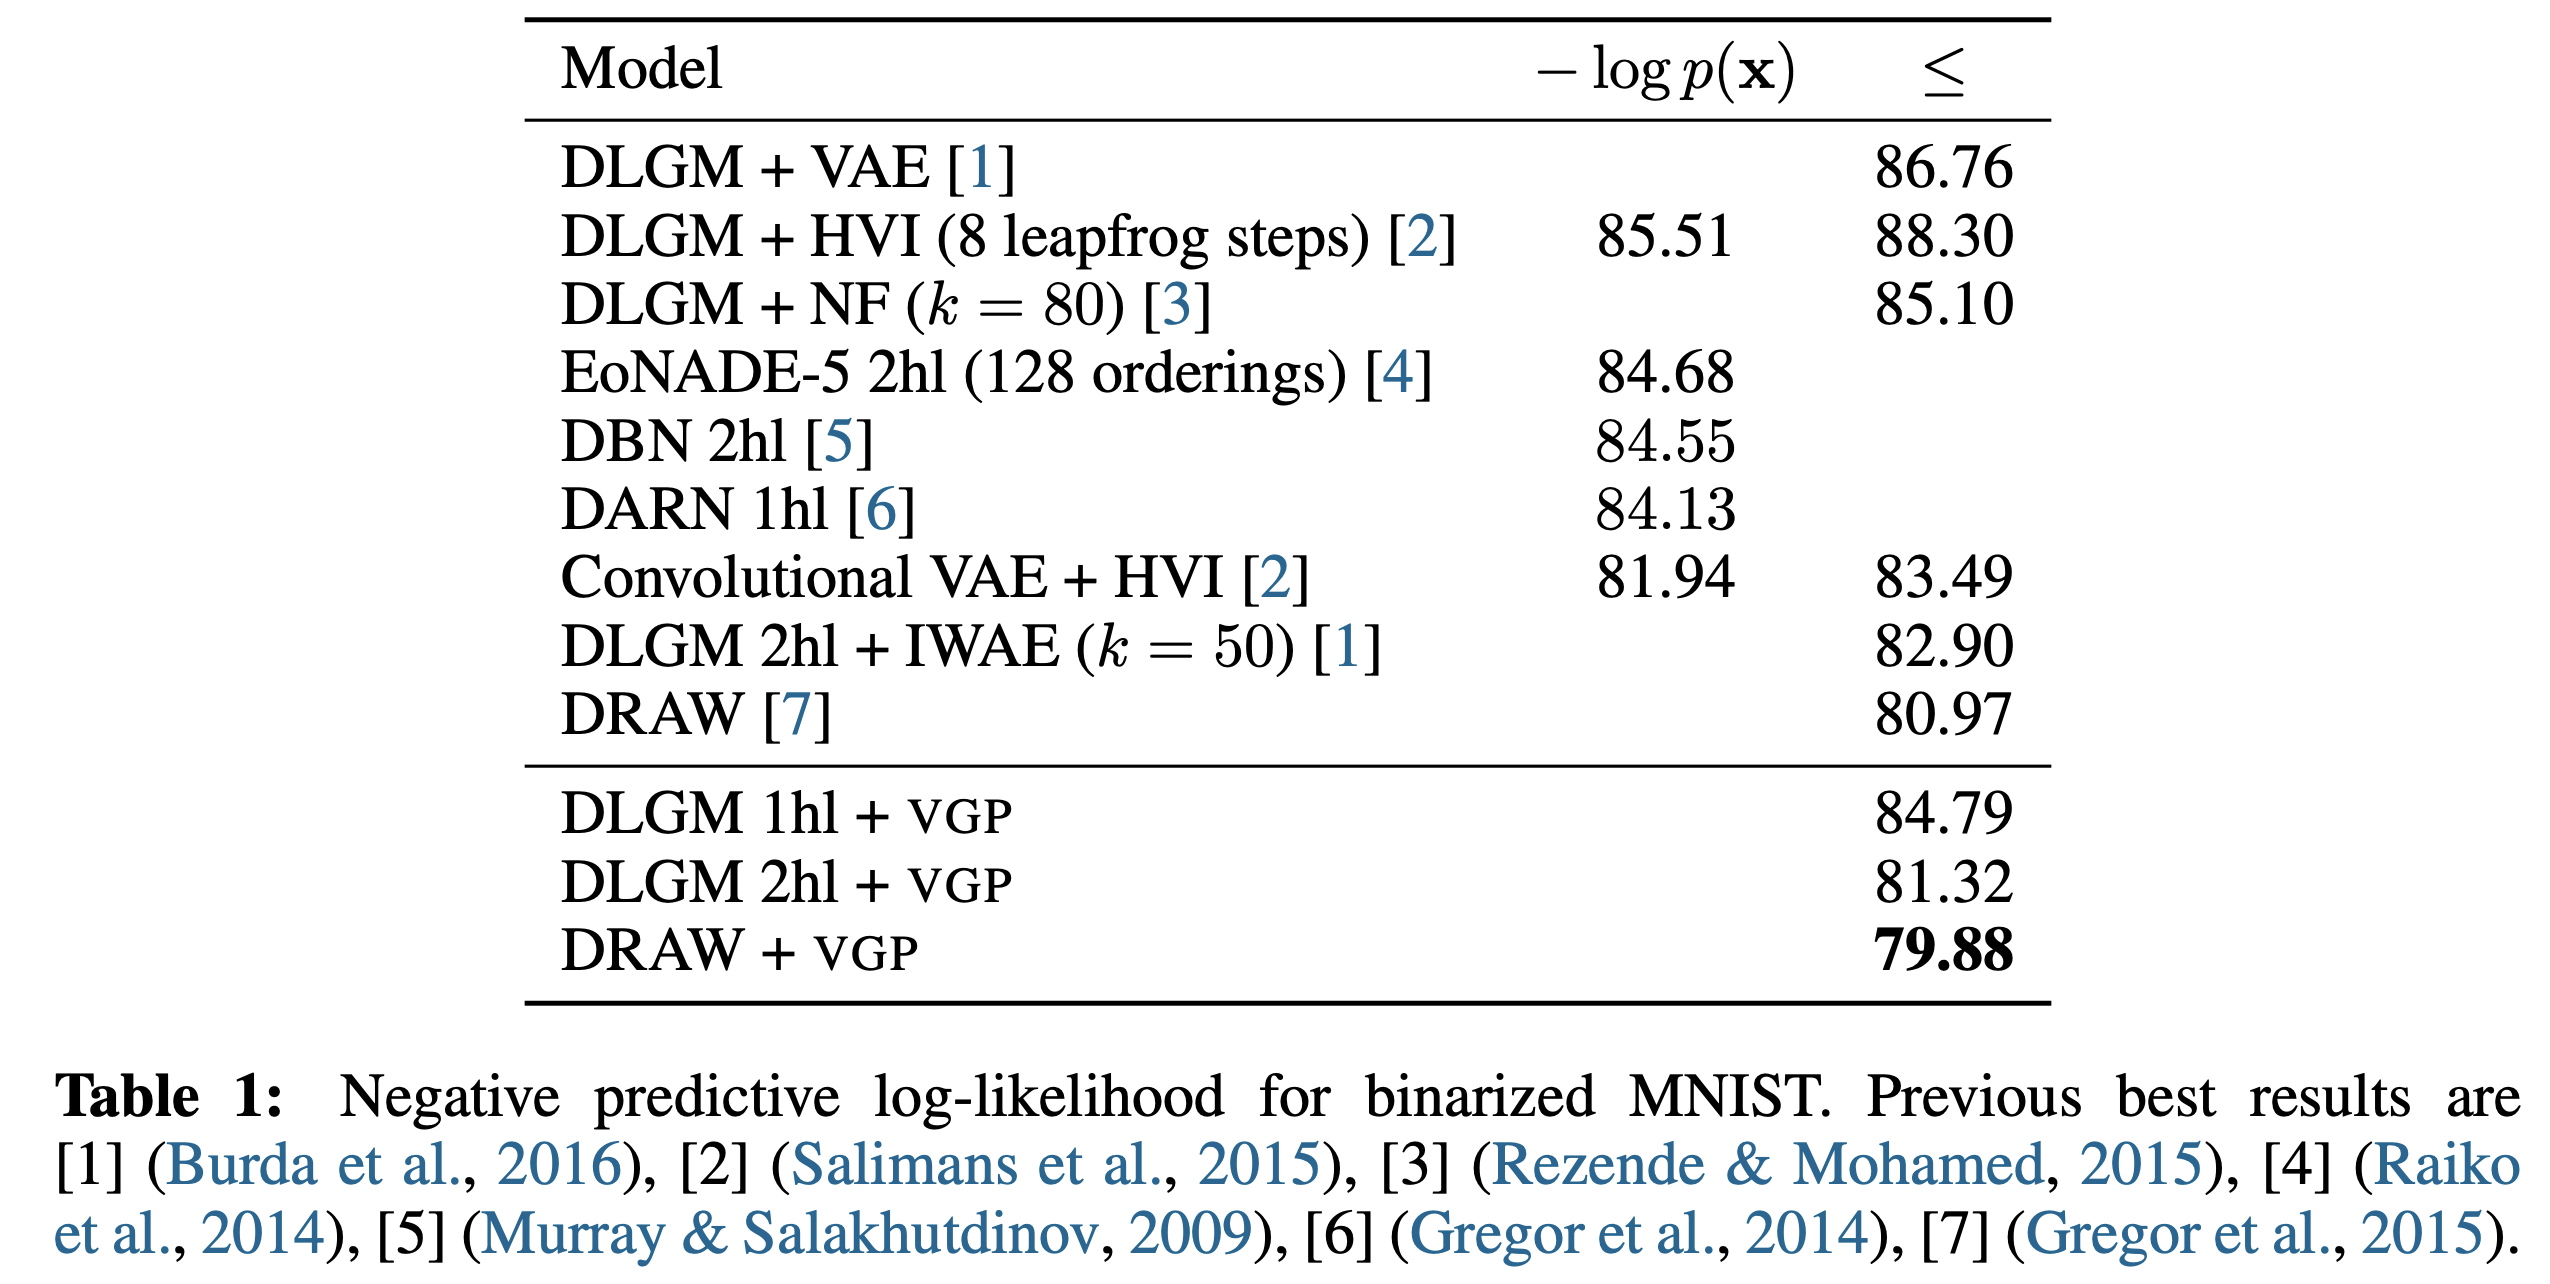
\includegraphics[scale=0.25]{images/table.png}
    \end{figure}
\end{frame}

\begin{frame}{Experiments}
    \begin{figure}{}
        \centering
        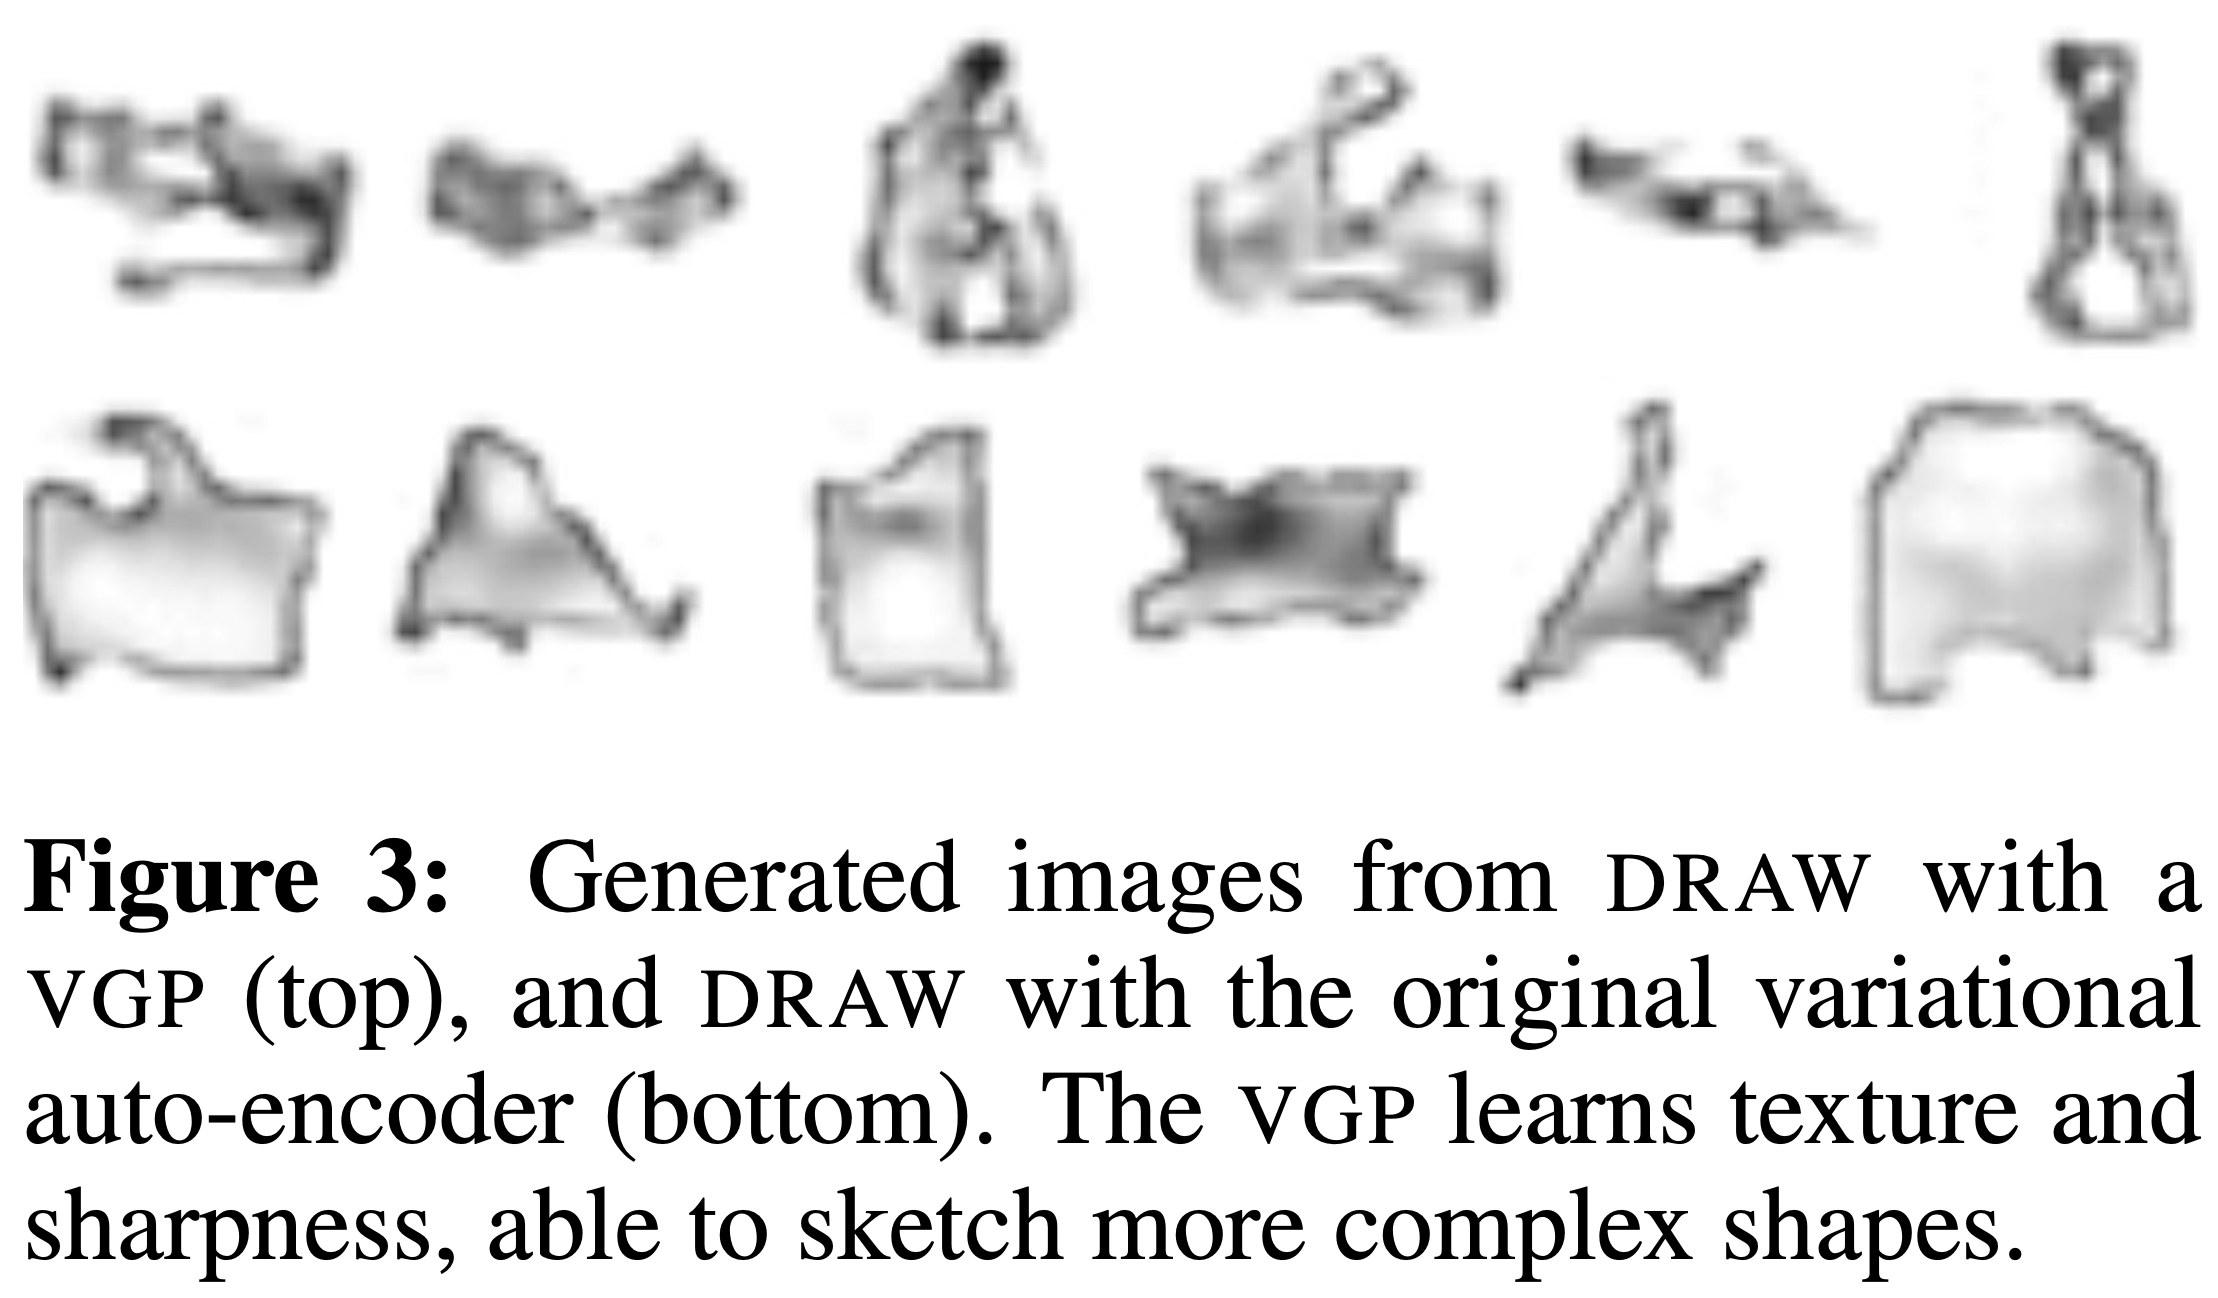
\includegraphics[scale=0.2]{images/figure3.png}
    \end{figure}

\end{frame}

\begin{frame}{Discussion}
    \begin{itemize}
        \item The VGP is a powerful variational model for approximating complex posterior distributions.
        \item Future work includes exploring VGP in Monte Carlo methods and characterizing local optima in the optimization procedure.
        \item The VGP shows promise for efficient and flexible inference in a variety of generative models.
    \end{itemize}
\end{frame}

\begin{frame}{Literature}
    \begin{enumerate}
        \item \textbf{Main article} \href{https://arxiv.org/pdf/1511.06499v4.pdf} 
        {The Variational Gaussian Process}
    \end{enumerate}
\end{frame}

\end{document}
